
\begin{figure}[ht!]
\centering
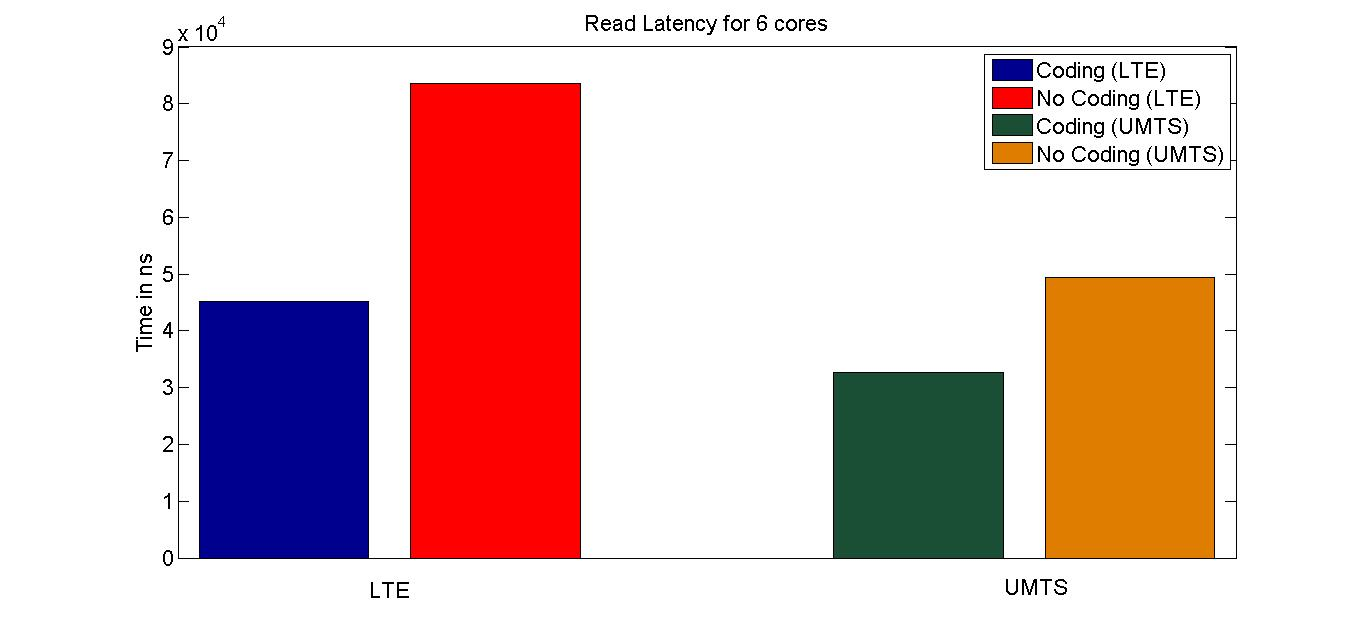
\includegraphics[width=500pt,natwidth=908,natheight=488]{LTE_vs_UMTS_edit.jpg}
\caption{Comparison of Coding vs No-Coding for UMTS and LTE}
\label{fig:lte_umts}
\end{figure}

\begin{itemize}
\item Figure~\ref{fig:lte_umts} shows an improvement of over 15$\%$ on both LTE and UMTS traces. As can be infered from the figure, the use of memory coding allows us to reduce the read latency by atleast $\mathbf{15\%}$.
\item The overhead of coding is divided in to memory overhead and control logic overhead. 
\item The memory overhead is dependent on the $\alpha$ fraction of memory which is coded using the dynamic coding scheme. 
\item For the given traces, $\alpha $ is approximately equal to $\mathbf{6\%}$ of the overall memory. 
\item The logical overhead is due to the scheduling of accesses for the use of coding banks at the memory controller. This may vary according to the specific implementation of the scheduling algorithm. 
\end{itemize}
Table~\ref{table:benefit_cost} presents the benefits and cost of each of the sub-scheme. It essentially presents the summary of the analysis done in the previous sections where we introduced each of these schemes. The condensed tabular format can be used to compare the cost and benefits of each of the sub-schemes. 
\begin{table}[ht!]
    \begin{tabular}{ | p{2cm} | p{7.5cm} | p{7.5cm} |}
    \hline
    Sub Scheme & Benefits (Per Region) & Costs \\ \hline
    Memory Coding &
    \vspace{-7mm}  
    \begin{itemize} 
    \item 10 reads Best case 
    \item 7 reads worst-worst case
    \item 2 writes per bank so 8 writes per region. Both for best case and worst case.
    \end{itemize}
    & 
    \vspace{-7mm} 
    \begin{itemize} 
    \item 1.5$\alpha$ times more memory.  
    \item control logic overhead for doing parallel reads and writes.
    \item Overhead of re-coding after a write. Each write needs a 3 reads and 4 writes.  
    \end{itemize}
 \\ \hline
    Dynamic Coding & 
    \vspace{-7mm} 
    \begin{itemize}
    \item Reduces the memory overhead to 5$\%$ in case of LTE. 
    \item Makes $\alpha$ to be 6$\%$ for UMTS. 
    \end{itemize}
    & 
    \vspace{-7mm} 
    \begin{itemize}
    \item Control logic for doing dynamic allocation. 
    \item Overhead of recoding during change of coded region. 
    \end{itemize}
 \\ \hline 
    Prefetching the codes & 
    Benefits more efficient reads & 
    Control logic for looking ahead in memory queue to prefetch the codes. 
 \\ \hline
    \end{tabular}
    \caption{Cost and Benefit of Coding scheme}
    \label{table:benefit_cost}
\end{table}
\\

\begin{comment}
\subsection{Simulation Setup}
\label{sec:simulation_setup}
To assess the performance increase of our coding scheme, we ran an analysis over the traces that closely resembled the coding polices that we have suggested, and 
compared them to the results when no coding scheme was implemented. The results of these tests can be seen in figure X. In our simulation, we made sure to run the create
the program with the worst case scenario for coding in mind. The following summarizes our scheme:

- We contain two queues for each of the banks, a write and a read queue. We assign a higher priority to read requests, unless the write queue fills up to a specific
set amount, in which case writes have a higher reuest. We always serve the oldest requests in the queue at any given time. In the case of a read, we first serve
the oldest request from its associated data bank. For all subsequent accesses during that cycle, we first determine if the request can be served by combining 
a previous request in addition to a parity bank. If so, then the current request is served from the parity bank. If not, then the request is served from the data bank.
In the case of a write, we first serve the oldest write present in the write queue to the data banks. If there is a bank conflict for any of the subsequent write
accesses, we then store the next write in the parity bank to avoid the conflict. We also consider the worst case scenario for writes, in which each write access 
takes 2 cycles. If a write for a memory location enters the queue and a previous write to the same location is still waiting in the queue, then the previous request
is dropped from the queue. Lastly, if there are still empty banks after serving all read or write requests from one of the queues, we then attempt to serve additional 
requests from the other queue. Our anlaysis shows that there is only a 0.6$\%$ space overhead to implement this for a 32 bit address space, and that one average the
clock cycle lateny is decreased by MORE THAN 15$\%$.
\end{comment}
